\lfoot{Autor: Daniel Melichar}
\subsubsection{Datenbankmanagementsysteme}
\label{subsec:dbms}

In der folgenden Sektion werden die gängisten RDBMS und NoSQL Datenbanken vorgestellt und gegeneinander Vergleicht. Es ist zu beachten, dass es ein wenig mehr zu NoSQL Datenbanken gibt, da wir mit einer solchen arbeiten (siehe \ref{subsec:datenmanagementimpl}).

\textbf{Relationale DBMS\newline}
\textbf{MySQL\newline}
Dieses RDBMS wurde ursprünglich entwickelt als \textit{lightweight database-like engine} und hatte in den ersten Versionen wenige von den Features die zu dem Zeitpunkt als essentiell gekennzeichnet waren. Trotz allem war es ein nützliches Tool, welches zwar kein eigentliches RDBMS war, aber dennoch einfach zum Einrichten und Verwenden war.

In den letzten Jahren ist MySQL von dem ursprünglichen Weg abgekommen – es hat sich zu einem kompletten RDBMS entwickelt.  Trotz Bekanntheit wird MySQL immer noch nicht als die stabilste Datenbank, oder jene mit dem größten Feature-Set, angesehen.

Alles im allen wird MySQL (oder Klone) in den meisten Fällen verwendet.

\textbf{Oracle\newline}
Dieses DBMS ist bekannt für seine große Anzahl an Features und dem größten Marktanteil. Vergleicht man Oracle mit anderen Datenbanken wird schnell klar, dass andere Datenbanken bei weitem nicht so viel können wie Oracle. Beinahe jedes Betriebssystem wird unterstützt; fast jede Programmiersprache hat Einbindungen die es ermöglichen mit einer Oracle Datenbank zu sprechen; Serverseite Programmierung hat viele Möglichkeiten; die Performance von Oracle Datenbanken ist exzellent; uvm.

Es gibt aber zwei große, negative Aspekte welche Oracle für viele nicht verwendbar machen: kosten und die Komplexität von Administration

\textbf{PostgreSQL\newline}
\todo{Content}

\textbf{SQL Server\newline}
\todo{Content}

\begin{table}[!htb]
\centering
\label{rdbms-comp}
\resizebox{\columnwidth}{!}{%
\begin{tabular}{|l|l|l|l|l|}
\hline
\textbf{Name} & \multicolumn{1}{c|}{\textbf{Microsoft SQL Server}} & \textbf{MySQL} & \textbf{Oracle} & \textbf{PostgreSQL} \\ \hline
\textbf{Website} & www.microsoft.com/sqlserver & www.mysql.com & www.oracle.com/database & www.postgresql.org \\ \hline
\textbf{Developer} & Microsoft & Oracle & Oracle & \begin{tabular}[c]{@{}l@{}}PostgreSQL Global\\ Development Group\end{tabular} \\ \hline
\textbf{\begin{tabular}[c]{@{}l@{}}Erster \\ Release\end{tabular}} & 1989 & 1995 & 1980 & 1989 \\ \hline
\textbf{\begin{tabular}[c]{@{}l@{}}Momentaner \\ Release\end{tabular}} & \begin{tabular}[c]{@{}l@{}}SQL Server 2014\\ April 2014\end{tabular} & \begin{tabular}[c]{@{}l@{}}5.7.11\\ February 2016\end{tabular} & \begin{tabular}[c]{@{}l@{}}12 Release 1 (12.1.0.2)\\ July 2014\end{tabular} & \begin{tabular}[c]{@{}l@{}}9.5.1\\ February 2016\end{tabular} \\ \hline
\textbf{Lizens} & Kommerziell & Open Source / Kommerziell & Kommerziell & Open Source \\ \hline
\textbf{\begin{tabular}[c]{@{}l@{}}Entwickelt\\ in..\end{tabular}} & C++ & C und C++ & C und C++ & C \\ \hline
\textbf{\begin{tabular}[c]{@{}l@{}}Unterstütze\\ Server\\ Systeme\end{tabular}} & Windows & \begin{tabular}[c]{@{}l@{}}FreeBSD\\ Linux\\ OS X\\ Solaris\\ Windows\end{tabular} & \begin{tabular}[c]{@{}l@{}}AIX\\ HP-UX\\ Linux\\ OS X\\ Solaris\\ Windows\\ z/OS\end{tabular} & \begin{tabular}[c]{@{}l@{}}FreeBSD\\ HP-UX\\ Linux\\ NetBSD\\ OpenBSD\\ OS X\\ Solaris\\ Unix\\ Windows\end{tabular} \\ \hline
\textbf{\begin{tabular}[c]{@{}l@{}}Unterstütze\\ Sprachen\end{tabular}} & \begin{tabular}[c]{@{}l@{}}.NET\\ Java\\ PHP\\ Python\\ Ruby\\ Visual Basic\end{tabular} & \begin{tabular}[c]{@{}l@{}}Ada\\ C\\ C\#\\ C++\\ D\\ Eiffel\\ Erlang\\ Haskell\\ Java\\ Objective-C\\ OCaml\\ Perl\\ PHP\\ Python\\ Ruby\\ Scheme\\ Tcl\end{tabular} & \begin{tabular}[c]{@{}l@{}}C\\ C\#\\ C++\\ Clojure\\ Cobol\\ Eiffel\\ Erlang\\ Fortan\\ Groovy\\ Haskell\\ Java\\ JavaScript\\ Lisp\\ Objective-C\\ OCaml\\ Perl\\ PHP\\ Python\\ R\\ Ruby\\ Scala\\ Tc\\ Visual Basic\end{tabular} & \begin{tabular}[c]{@{}l@{}}.NET\\ C\\ C++\\ Java\\ Perl\\ Python\\ Tcl\end{tabular} \\ \hline
\textbf{\begin{tabular}[c]{@{}l@{}}APIs und \\ andere Verbindungs-\\ möglichkeiten\end{tabular}} & \begin{tabular}[c]{@{}l@{}}OLE DB\\ Tabular Data Stream (TDS)\\ ADO.NET\\ JDBC\\ ODBC\end{tabular} & \begin{tabular}[c]{@{}l@{}}ADO.NET\\ JDBC\\ ODBC\end{tabular} & \begin{tabular}[c]{@{}l@{}}ODP.NET\\ Oracle Call Interface (OCI)\\ JDBC\\ ODBC\end{tabular} & \begin{tabular}[c]{@{}l@{}}Native C Libary\\ ADO.NET\\ JDBC\\ ODBC\end{tabular} \\ \hline
\end{tabular}
}
\caption{Vergleich von relationalen Datenbankmanagementsystemen \cite{MELD.CH2-dbms.compRDBMS}}
\end{table}

\clearpage

\textbf{NoSQL Datenbanken\newline}

Im allgemeinen gibt es vier Arten von NoSQL Datenbanken\cite{MELD.CH2-dbms.compNoSQLInfo}: Key-Value Stores, Column-Oriented Databases, Document Databases und Graph Stores. Selbstverständlich gibt es auch eigens entwickelte Datenbanken die nicht in diese vier Kategorien eingeteilt werden können, diese vier sind aber jene die am meisten verwendet werden.

\begin{itemize}
	\item \textbf{Key-Value Stores\newline}
	Diese Art von Datenbank ist prinzipiell ziemlich simple, aber dennoch effizient und schnell. In den meisten Fällen kommuniziert man mit der Datenbank mittels einer API die für mehrere Programmiersprachen zur Verfügung gestellt wurde. In den meisten Fällen wird der Key mittels Strings realisiert und dieser referenziert auf die Values (also die eigentlichen Daten). Diese Datenbanken sind Hash-Tabellen sehr ähnlich, da auch hier der Key als Index verwendet wird und somit schnelle Zugriffszeiten ermöglicht werden. Wie bei den meisten NoSQL Datenbanken ist auch bei Key-Value kein Schema aufzufinden.

	Beispielhafte Anwendungen von Key-Value Datenbaken wären die Speicherung von Session Daten eines Users, die Speicherung der Artikel in einem Einkaufswagen, oder die Speicherung der beliebten Produkte.

	Bekannte Key-Value Datenbanken: Amazon DynamoDB und RIAK

	\begin{figure}[!htb]\centering
		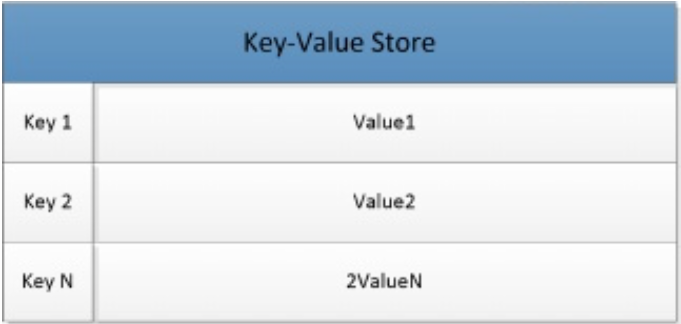
\includegraphics[width=0.5\textwidth]{images/keyvalueStore}
		\caption{Aufbau von Key-Value Datenbanken}
	\end{figure}

	\clearpage

	\item \textbf{Column-Oriented Databases\newline}
	Column Stores in NoSQL sind eigentlich eine Mischung aus Row/Column Stores anders als bei relationalen column Datenbanken. Es herrscht zwar das selbe Konzept von Zeile-nach-Zeile wie bei relationalen Datenbanken, aber diese werden nicht in Tabellen gespeichert, sondern in massiven, verteilten Architekturen. Jeder Key ist mit einer oder mehreren Attributen verknüpft. Diese Art von Datenbank ist grundsätzlich so aufgebaut das mit einem einzigen Befehl eine große Menge an Daten zurückgebracht werden kann. 

	Column Store Datenbanken werden sehr oft für Data Mining, Datawarehousing und im Allgemeinen für Business Analytics verwendet.

	Einige der Bekanntesten Datenbanken sind: Googe BigTable, Cassandra

	\begin{figure}[!htb]\centering
		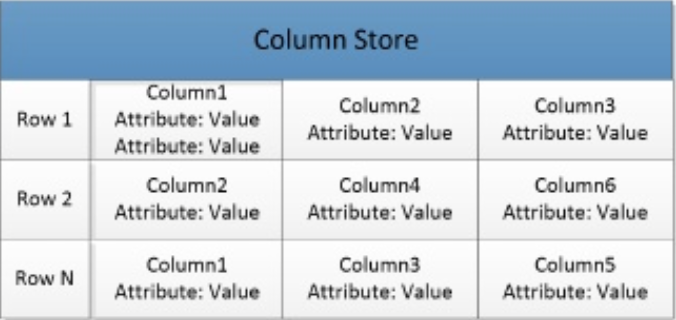
\includegraphics[width=0.5\textwidth]{images/columnStore}
		\caption{Aufbau von Column-Oriented Datenbanken}
	\end{figure}

	\clearpage

	\item \textbf{Document Databases\newline}
	Document Store Database sind jene Datenbanken die Daten in Form von Files ablegen und speichern. Hierbei ist vor allem auf die Performance und horizontale Skalierbarkeit zu achten. Die Files, oder Dokumente, in einer Document-Oriented Datenbank sind ähnlich zu jenen einer relationalen Datenbank, aber der große Unterschied hierbei ist, dass diese an kein Schema gebunden sind und somit um einiges flexibler sind. Es werden oftmals standardisierte Formate wie XML, PDF oder JSON verwendet. Diese Dokumente sind mittels einem eindeutigen Key adressiert welcher das File auch repräsentiert. Diese Keys können einfache Strings oder ganze Pfade sein.

	Anwendungsgebiete von dieser Art von Datenbank sind Applikationen wie Content Management Systeme, Blog Software, usw. 

	Die bekanntesten Document-oriented Datenbanken sind: MongoDB und CouchDB

	\begin{figure}[!htb]\centering
		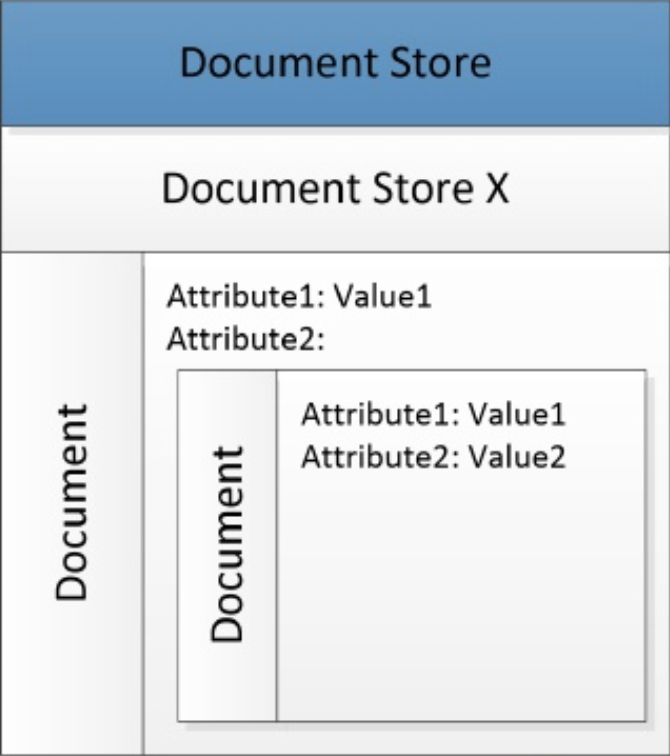
\includegraphics[width=0.5\textwidth]{images/documentStore}
		\caption{Aufbau von Document Datenbanken}
	\end{figure}

	\clearpage

	\item \textbf{Graph Stores\newline}
	In Graph Datenbanken werden die Daten mittels so genannten Nodes und Edges gespeichert, wobei Nodes als Objekte arbeiten und Edges und die Beziehungen zwischen den einzelnen Objekten. Es wird hier die \textit{Index-Free-Adjacency} Technik verwendet. Das bedeutet, dass jeder Node mit Pointern versetzt wurde die es ermöglichen auf den nächstgelegenen Node zugriff zu bekommen. Somit kann mit einem Befehl über mehrere Nodes iteriert werden. In Graph-Oriented Datenbanken liegt der Hauptsächliche Fokus auf die Verbindung zwischen den Daten, also in welcher Beziehung diese stehen. Anders als bei anderen NoSQL Datenbanken wird bei Graph Datenbanken oftmals teile des ACID Models verwendet.

	Sozialle Netzwerke sind die hauptsächlichen Anwendungsgebiete von Graph Datenbanken, aber auch Applikationen für Sicherheits- und Zugriffskontrollen, Content Management Systeme, Cloud Management, etc. 

	Die am verbreitete Graph Datenbank ist ohne Zweifel Neo4j

	\begin{figure}[!htb]\centering
		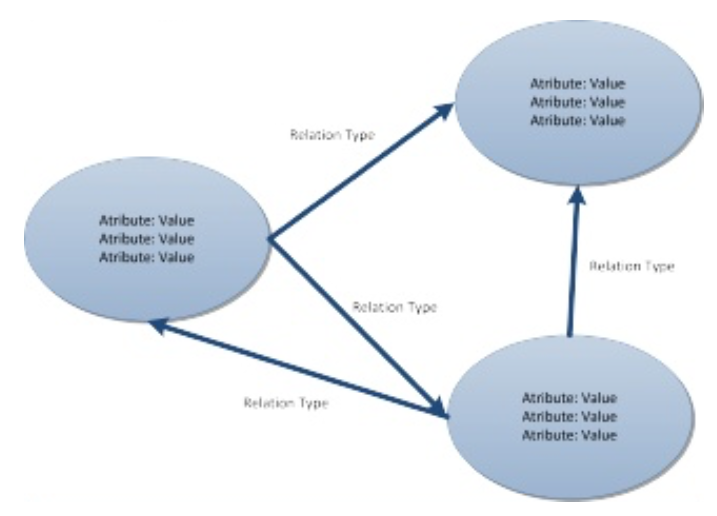
\includegraphics[width=0.5\textwidth]{images/graphStore}
		\caption{Aufbau von Document Datenbanken}
	\end{figure}
\end{itemize}
\clearpage

Hier kann man nochmalsd jene NoSQL Datenbanken betrachten und vergleichen die zum hautigen Zeitpunkt am meisten verwendet werden.

\begin{figure}[!htb]\centering
	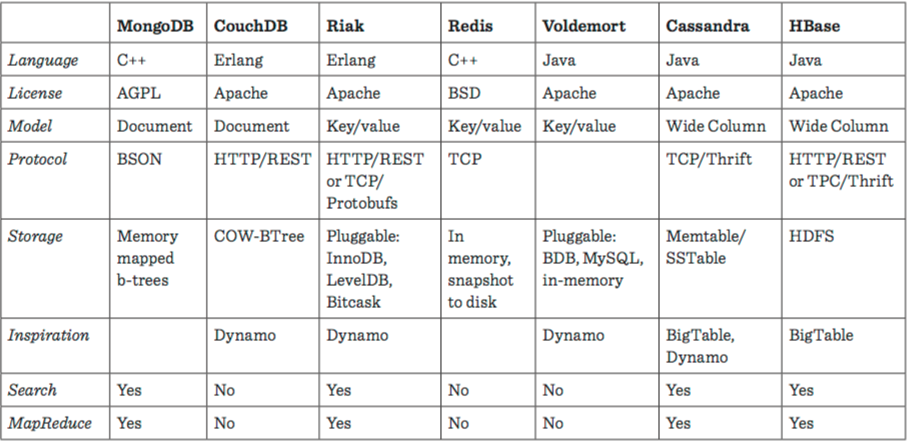
\includegraphics[width=1\textwidth]{images/noSQLComp}
	\caption{Vergleich von gängigen NoSQL Datenbanken\cite{MELD.CH2-dbms.compNoSQL}}
\end{figure}


\clearpage % DO NOT REMOVE